\section{Deroulement de la partie}
\subsection{Tours de jeu}
Une partie dure jusqu'à ce qu'une des conditions de fin de partie soit remplie.
Ces conditions inclues, mais ne sont pas limitées à :
\begin{itemize}
  \item L'épuisement du compteur de tours.
  \item Tout les adversaires d'un joueur sont mort (ils ne disposent plus d'unité).
\end{itemize}
Le nombre de tours est directement implémenté dans le GameManager, et est testé à chaque tour de jeu.
L'autre condition est testée après chaque mouvement. On veut ainsi être certain que la partie se termine dès qu'un seul joueur est encore vivant.
On peut bien sur imaginer d'autres conditions, telles que la prise d'une case particulière ou la mort d'une certaine unitée.
Ces conditions sont implémentables dans l'architecture actuelle car un changement dans l'état du jeu implique qu'il y ait eu un mouvement ou une fin de tour, les deux cas où l'on teste les conditions de fin de partie.
\newline
Le déroulement de la partie est classique : les joueurs jouent chacun leur tour, bougent leurs unités tant qu'elles disposent de mouvement et décident quand ils veulent terminer leur tour (possiblement car il ne peuvent plus faire d'actions).
Ce déroulement de la partie est détaillé davantage sur le diagramme de séquence \ref{fig:gameFlow}.
\begin{figure}[h!]
    \centering
    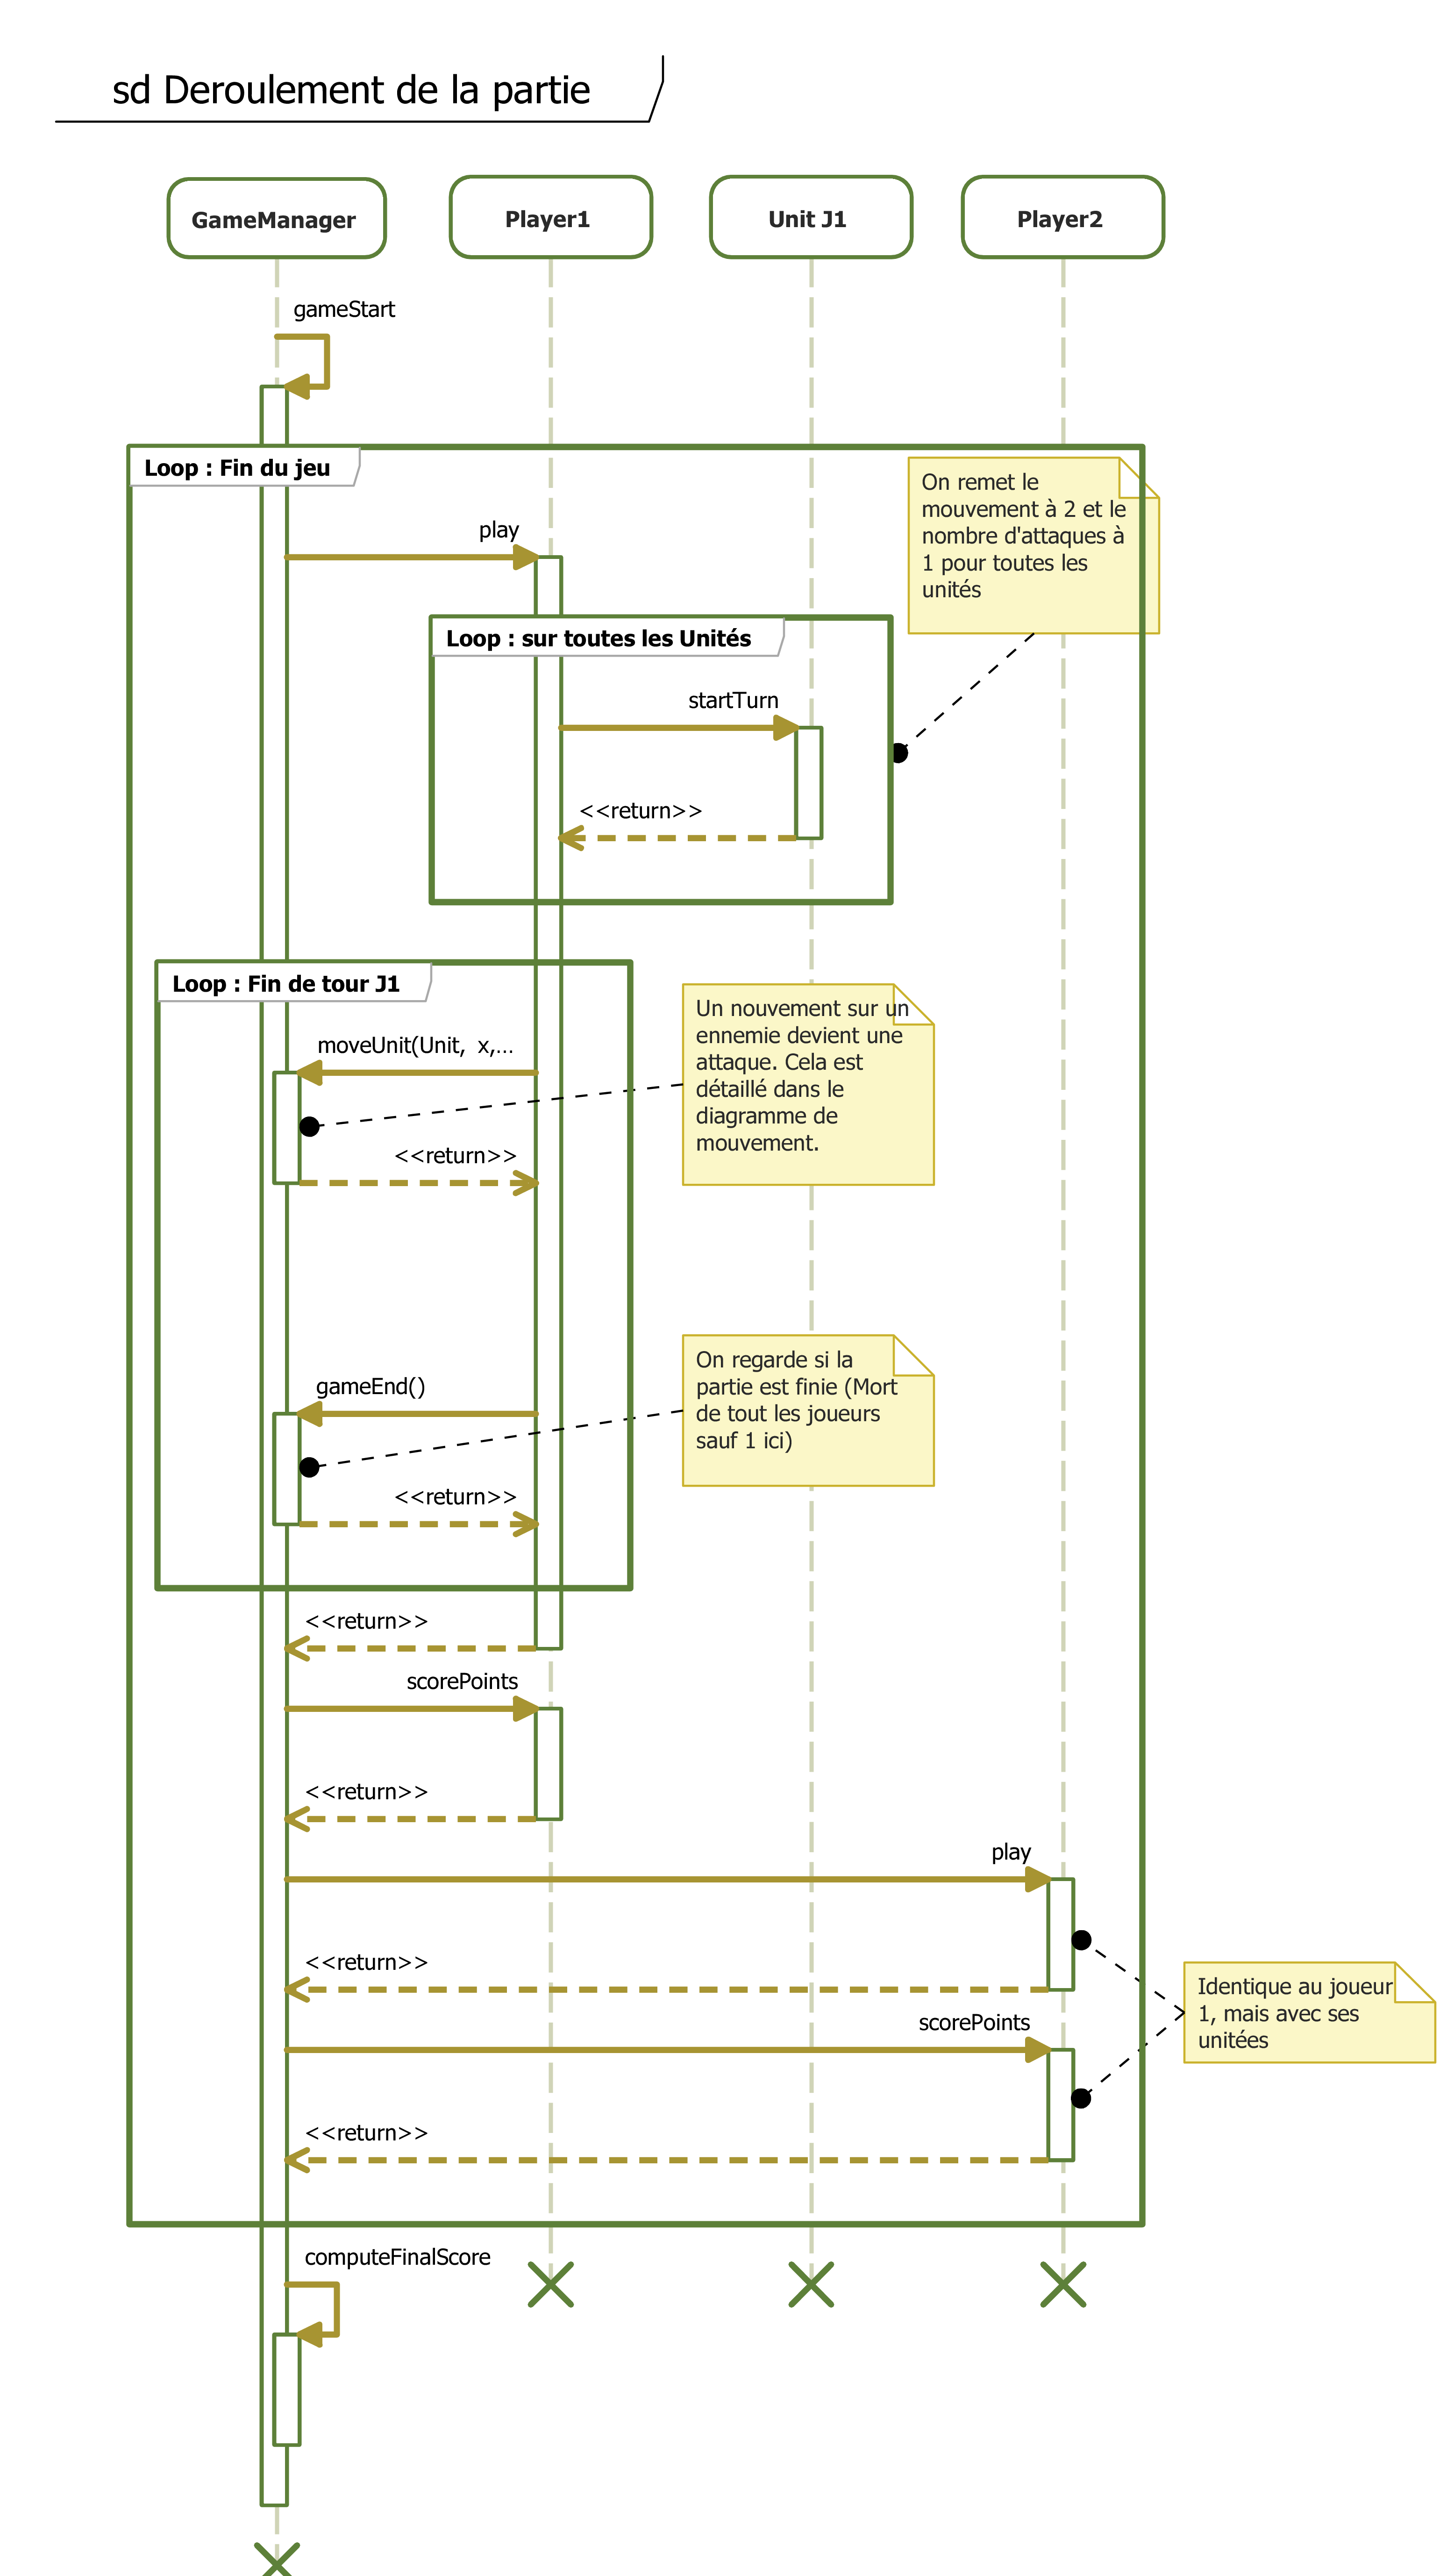
\includegraphics[width=0.8\textwidth]{res/DeroulementPartie.png}
    \caption{Deroulement de la partie}
    \label{fig:gameFlow}
\end{figure}

\subsection{Mouvements et attaques}
La fonctionnalité d'attaque est incluse dans un mouvement. 
Si une unité se déplace sur une case où se trouve une ou plusieurs unités adverse, la procédure de combat est lancée.
De ce fait, l'interface graphique n'aura qu'a implémenter uniquement le contrôle sur le déplacement, et pas sur l'attaque.
\newline
Les combats sont réalisés séquentiellement eux aussi; l'attaquant attaque toujours au défenseur le plus fort, et lui porte un nombre d'attaque égal au nombre de points de vie de l'unité le plus important plus deux.
Il y a donc toujours au minimum 3 attaques de prévues contre une unité. Le combat peut bien sur se terminer plus tôt si l'une des deux venait à mordre la poussière !
\'A la fin d'un combat, le gestionnaire de jeu teste si l'une des unités est morte (et donc la fin potentielle du jeu) et demande au joueur de la retirer de sa liste d'unités valides.
Ce fonctionnement est détaillé davantage sur le diagramme de séquence \ref{fig:movement}.
\begin{figure}[h!]
    \centering
    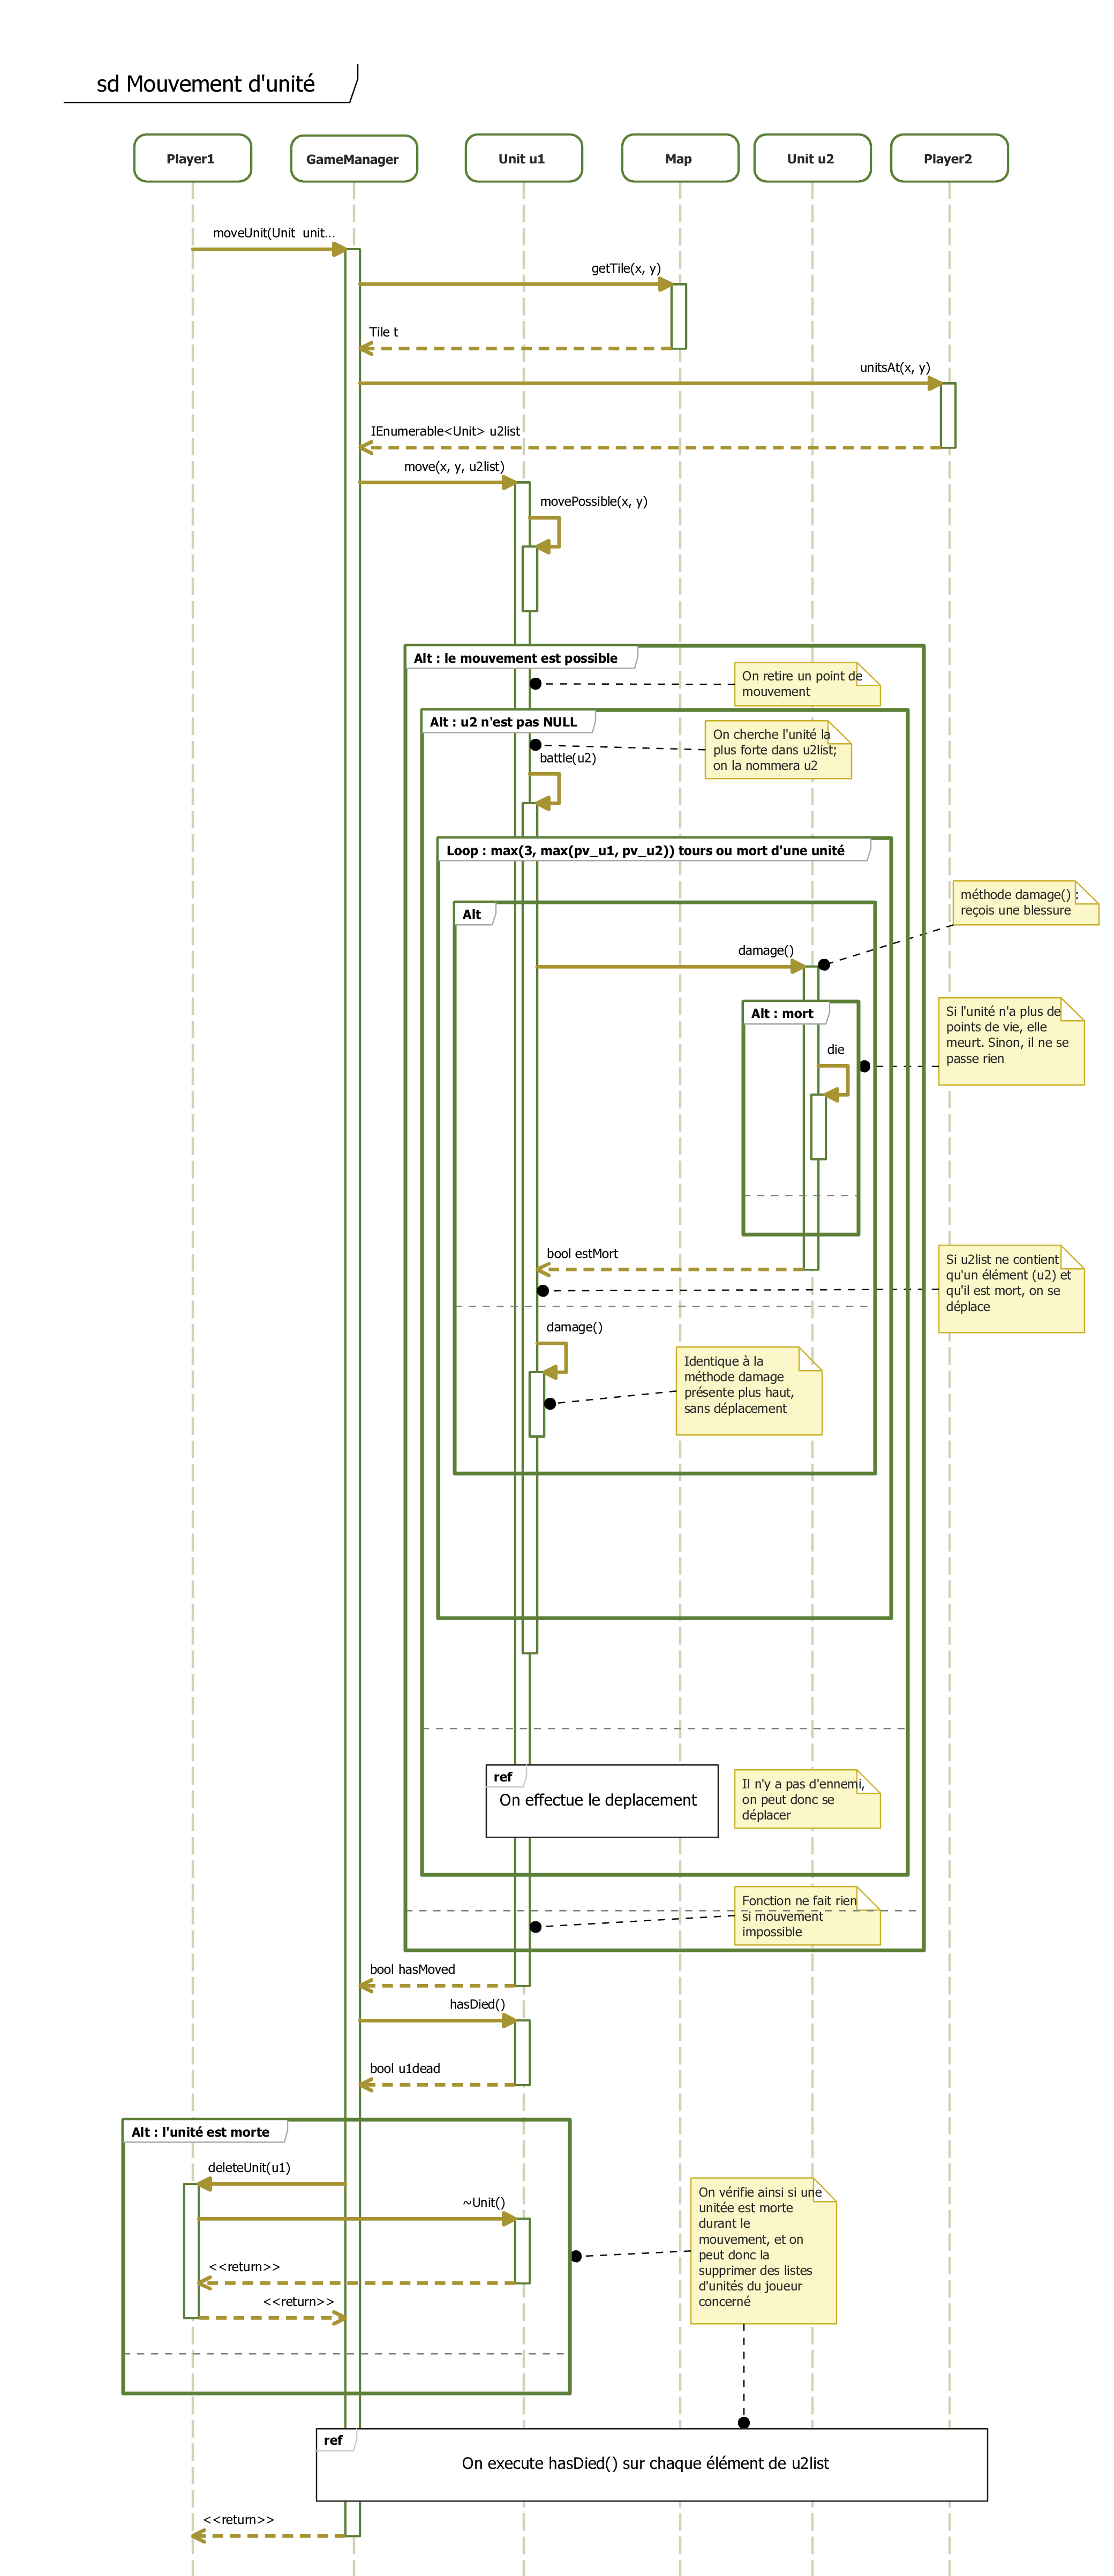
\includegraphics[width=0.7\textwidth]{res/MouvementUnite.png}
    \caption{Mouvement et combat}
    \label{fig:movement}
\end{figure}

\subsection{Activité sur une case}
Nous l'avons compris, les cases sont le nef de la guerre.
Il est en effet très difficile de gagner sans contrôler les bonnes cases.
Une première approche stratégique pourrait être de controler un maximum de cases par exemple; il est donc très important d'être bien au fait de \textit{l'état de la case}.
Une case a trois états :
\begin{itemize}
  \item Libre, c'est à dire avec aucune unité dessus.
  \item Contrôlé par le joueur (il dispose au moins d'une unité dessus).
  \item Contrôlé par l'adversaire (même condition).
\end{itemize}
L'état d'une case change suivant si un joueur la quitte ou se la fait prendre.
Cet état n'est donc dépendant uniquement des déplacements et attaques des joueurs, et pas de l'état du jeu (tour actuel...).
Davantage de détails sont disponibles dans le diagramme d'états-transitions \ref{fig:CaseOccupation}.
\begin{figure}[h!]
    \centering
    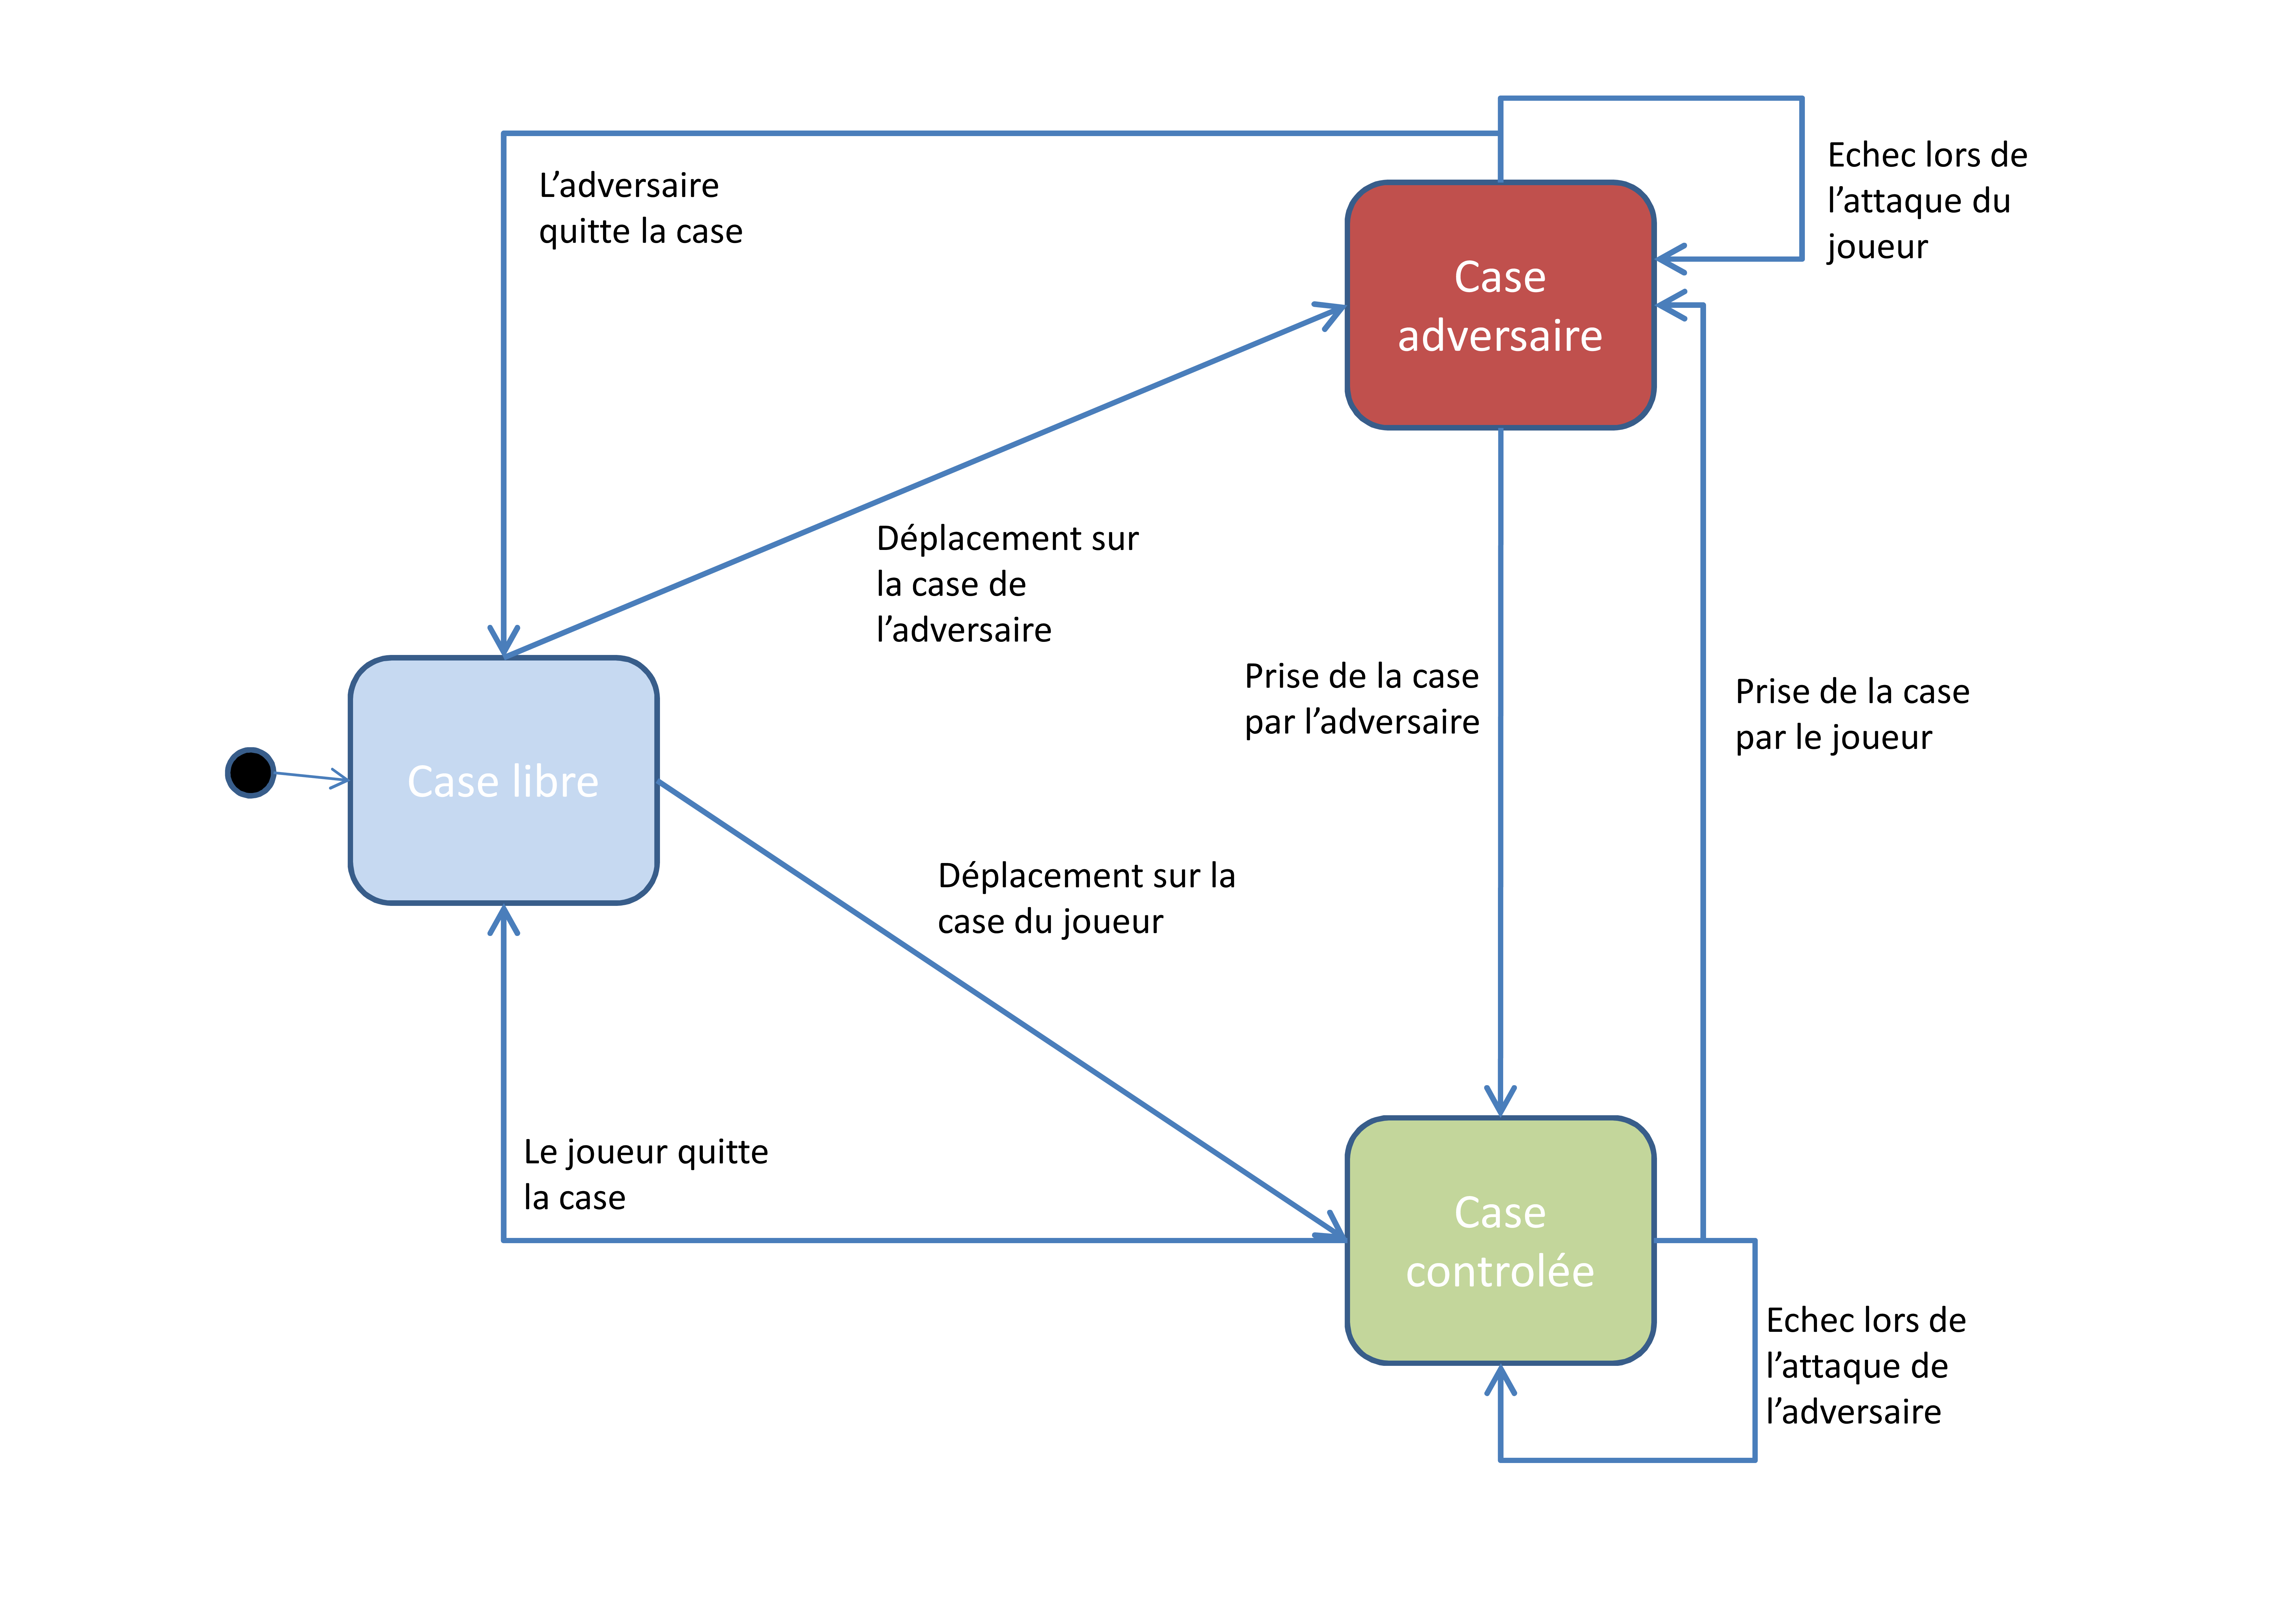
\includegraphics[width=0.8\textwidth]{res/OccupationCase.png}
    \caption{Occupation d'une case de jeu}
    \label{fig:CaseOccupation}
\end{figure}
L'une des particularités de ce projet sont les cases hexagonales.
Elles ne présentent pas de véritables soucis d'implémentation car les équations de mouvement sont facilement modélisables mathématiquement.
En effet, les cases adjacentes ont pour indice (X-a, Y-b) avec a et b égaux à 0, 1 ou -1.
On remarquera cependant que les cases hexagonales disposent de 6 cotés contre 4 pour les cases carrés.
On peut dons s'attendre à des parties plus animées car il est plus rapide sur un plateau hexagonal de déplacer d'un coin à l'autre du plateau.